\documentclass[9pt,twocolumn,twoside]{pnas-new}

% -- Template Setup --
\templatetype{pnasresearcharticle}
\articletype{SOCIAL SCIENCES}

% =============================================================
%  NUCLEAR PATCH: REMOVE LINE NUMBERS & WATERMARK
% =============================================================
\makeatletter
% Disable line numbers and watermark in this template
\renewcommand{\linenumbers}{}
\setboolean{displaywatermark}{false}
\makeatother
% =============================================================

% -- Essential Packages --
\usepackage{booktabs}
\usepackage{microtype}
\usepackage{graphicx}

\title{Network, Language, and Sentiment in \emph{Game of Thrones} Season~1}

% -- Author & Affiliation --
\author[a,1]{Bashar Bdewi}
\affil[a]{Technical University of Denmark (DTU), Department of Applied Mathematics and Computer Science, 2800 Kongens Lyngby, Denmark}

\leadauthor{Bdewi}

% -- Corresponding Author --
\correspondingauthor{\textsuperscript{1}To whom correspondence should be addressed. E-mail: basharbdewi86@gmail.com}

% -- Significance Statement --
\significancestatement{Complex TV series like \emph{Game of Thrones} are built around dense webs of characters, alliances, and conflicts. This paper combines social network analysis and classical NLP on Season~1 dialogue to show how narrative roles, faction structure, and emotional tone emerge directly from the script. We construct an interaction network between characters, detect communities, and analyze the language and sentiment of each group using TF--IDF and the LabMT happiness lexicon. The results demonstrate that a simple, transparent pipeline---usable in a classroom setting---can recover major factions (Starks, Lannisters, Night's Watch, Dothraki) and quantify how their language differs in topic and emotional valence. This illustrates how network and text tools can be used to study storytelling at scale.}

% -- Author Contributions --
\authorcontributions{B.B.\ designed the research, implemented the data processing and analysis pipeline, produced all figures, and wrote the manuscript.}

% -- Declaration --
\authordeclaration{The author declares no competing interests.}

% -- Keywords --
\keywords{Social networks $|$ Community detection $|$ Text mining $|$ Sentiment analysis $|$ Game of Thrones}

% -- Abstract --
\begin{abstract}
Narrative worlds in popular TV series offer rich testbeds for social network and text analysis. In this study, I analyze Season~1 of the HBO series \emph{Game of Thrones} using a joint network--and--text pipeline aligned with the DTU course 02805 \emph{Social Graphs and Interactions}. From a public script dataset, I construct an undirected, weighted character interaction network where nodes are characters and edges connect speakers who exchange dialogue within a scene. Using NetworkX, I compute global statistics, centrality measures, and Louvain communities. I then aggregate dialogue by community, apply TF--IDF and wordclouds to identify lexical themes, and estimate community-level sentiment using the LabMT happiness lexicon. The Season~1 network contains 146 characters and 482 edges in a single giant component. Degree, betweenness, and eigenvector centralities highlight Eddard Stark, Catelyn Stark, Tyrion Lannister, and Cersei Lannister as structural hubs and brokers, broadly consistent with their narrative importance. Louvain communities correspond to meaningful factions such as the Winterfell/Stark cluster, King’s Landing politics, the Night’s Watch at the Wall, and Daenerys’s Dothraki storyline. TF--IDF and wordclouds show that each community is characterized by distinct vocabulary related to setting and plot. LabMT sentiment scores reveal small but systematic differences in emotional tone between communities, with political and war-focused groups displaying slightly lower average happiness. Overall, the pipeline demonstrates how standard tools from network science and NLP can be combined into a compact, interpretable project that connects course concepts to a popular cultural domain.
\end{abstract}

% -- Dates & DOI --
\dates{This manuscript was compiled on \today}
\doi{\url{https://doi.org/10.0000/xxx}}

\begin{document}

\maketitle
\thispagestyle{firststyle}
\ifthenelse{\boolean{shortarticle}}{\ifthenelse{\boolean{singlecolumn}}{\abscontentformatted}{\abscontent}}{}

%%%%%%%%%%%%%%%%%%%%%%%%%%%%%%%%%%%%%%%%%%%%%%%%%%%%
% Introduction
%%%%%%%%%%%%%%%%%%%%%%%%%%%%%%%%%%%%%%%%%%%%%%%%%%%%

\section*{Introduction}

Television series with large casts and long-running story arcs provide natural laboratories for studying complex social systems. Characters form alliances and rivalries, information spreads through conversations, and communities emerge around families, locations, and political factions. Social network analysis offers tools to quantify these structures~\cite{newman2010,barabasi2016}, while natural language processing (NLP) can reveal what different groups talk about and how they feel about their world~\cite{bird2009}.

\emph{Game of Thrones} (GoT) is particularly well suited to this kind of analysis. Several authors have already shown that the underlying universe of books and TV episodes can be represented as a social network with nontrivial structure and interpretable communities~\cite{beveridge2016,liu2017}. These studies typically focus either on graph structure alone (centralities, assortativity, structural balance) or on textual features extracted from the novels.

In contrast, this paper aims at a compact, course-aligned project that integrates the main elements of the DTU 02805 \emph{Social Graphs and Interactions} syllabus:

\begin{itemize}
    \item Network construction and basic statistics,
    \item Centralities and community detection,
    \item Classical NLP with NLTK and TF--IDF,
    \item Sentiment analysis using the LabMT lexicon ~\cite{dodds2011}.
\end{itemize}

Using a public script dataset for the TV show~\cite{gotkaggle}, I focus on Season~1 and construct an undirected character interaction network, where edges connect characters who speak to each other within the same scene. I then ask three guiding questions:

\begin{enumerate}
    \item How does the Season~1 interaction network look at the global level (size, density, connected components, degree distribution)?
    \item Which characters emerge as structurally important according to degree, betweenness, and eigenvector centrality, and how does this compare to their narrative roles?
    \item Do communities discovered in the interaction network correspond to narrative factions, and do they differ in both lexical themes and sentiment?
\end{enumerate}

By answering these questions in a unified pipeline, I demonstrate that a straightforward combination of NetworkX, NLTK, scikit-learn, and LabMT yields a coherent research finding: \emph{network structure, language, and sentiment all align with the main factions and storylines of Season~1}.

%%%%%%%%%%%%%%%%%%%%%%%%%%%%%%%%%%%%%%%%%%%%%%%%%%%%
% Results
%%%%%%%%%%%%%%%%%%%%%%%%%%%%%%%%%%%%%%%%%%%%%%%%%%%%

\section*{Results}

\subsection*{Global structure of the Season~1 network}

From the script dataset, I extract all Season~1 lines and construct an undirected, weighted network in which each node represents a unique speaker name and edges connect pairs of speakers who exchange at least one line within a scene. Multiple exchanges increase the edge weight. After cleaning speaker names and removing self-loops, the Season~1 network contains 146 nodes and 482 edges. The graph is connected: all characters belong to a single giant component. The edge density is approximately 0.046, indicating a sparse but not extremely fragmented network.

The degree distribution is right-skewed: most characters have low degree, while a small number of hubs interact with many others. This qualitatively matches expectations for narrative networks~\cite{newman2010}. Figure~\ref{fig:network} shows the Season~1 interaction graph with node size proportional to eigenvector centrality and colors indicating communities (discussed below).

\begin{figure*}[t!]
    \centering
    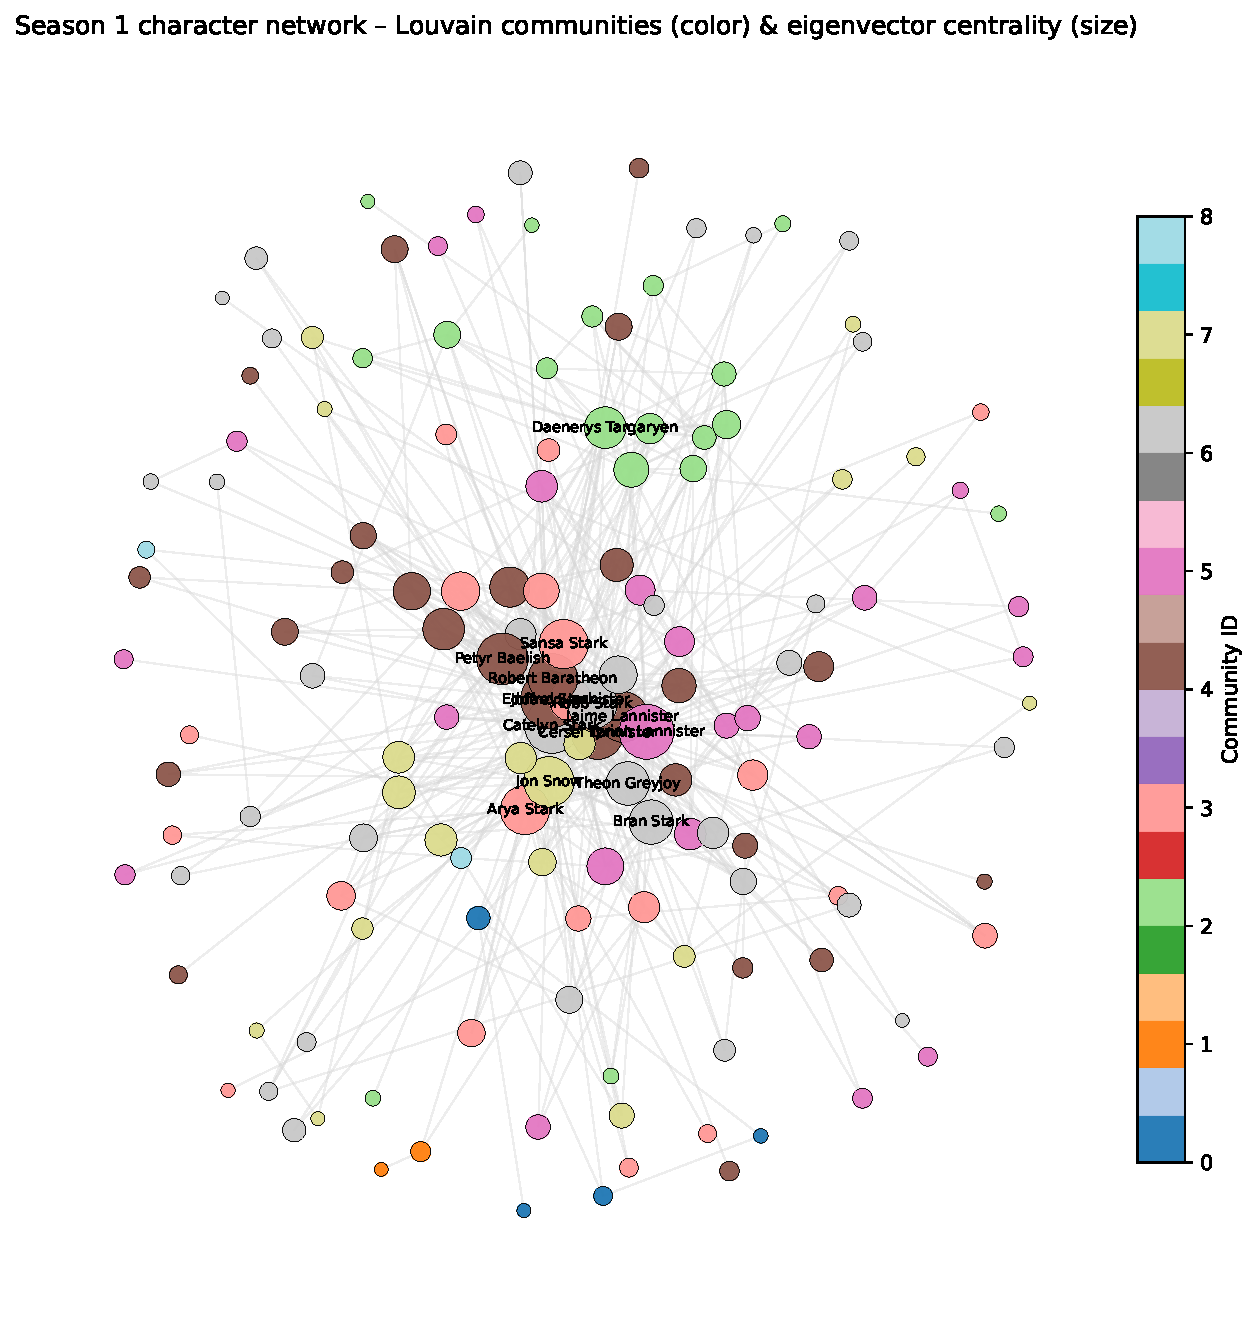
\includegraphics[width=0.9\textwidth]{fig_network.pdf}
    \caption{Season~1 character interaction network. Nodes are colored by Louvain community and sized by eigenvector centrality. The layout shows clear clusters corresponding to main narrative factions (Winterfell, King’s Landing, the Wall, and the Dothraki storyline).}
    \label{fig:network}
\end{figure*}

\subsection*{Central characters and narrative roles}

I compute degree, betweenness, and eigenvector centrality for all characters using NetworkX~\cite{hagberg2008}. All three measures highlight a similar set of structurally important characters: Eddard Stark, Catelyn Stark, Tyrion Lannister, Cersei Lannister, Robert Baratheon, Jon Snow, and Robb Stark are consistently ranked near the top.

Eddard Stark has the highest degree centrality and one of the highest betweenness scores, consistent with his role as the main connector between Winterfell and King’s Landing plots. Tyrion Lannister and Cersei Lannister also show high betweenness, reflecting their roles as brokers in the political core. Jon Snow appears as a central node in the Night’s Watch subgraph, with high degree and eigenvector centrality within that region.

Figure~\ref{fig:centralities} summarizes the top-10 characters by degree, betweenness, and eigenvector centrality. The overlap between these lists matches narrative expectations: characters that dominate screen time and drive major decisions also occupy structurally privileged positions in the interaction network.

\begin{figure*}[t!]
    \centering
    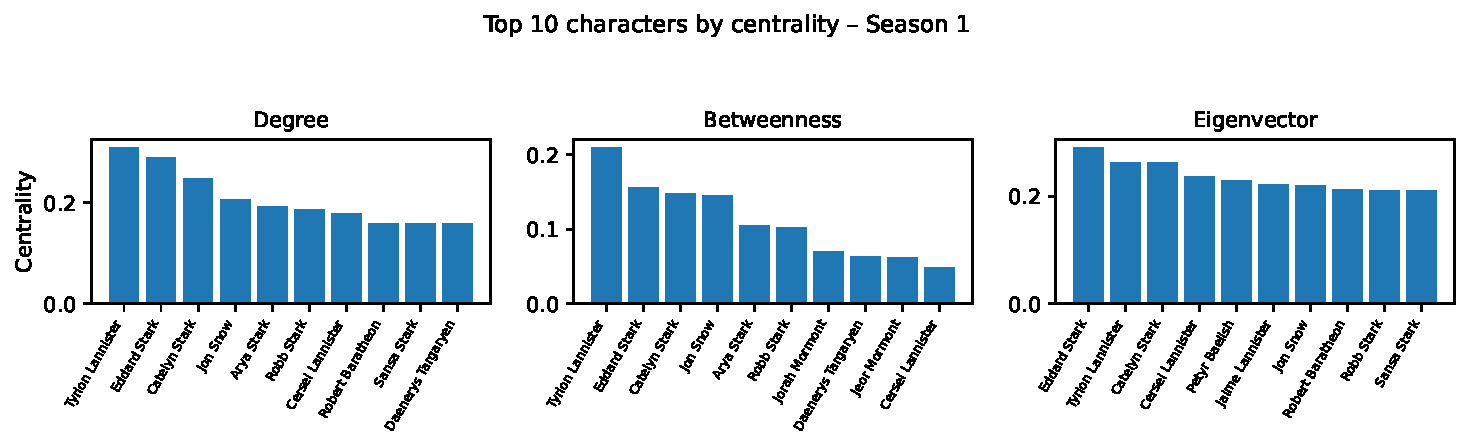
\includegraphics[width=0.9\textwidth]{fig_centralities.pdf}
    \caption{Centrality ranking of Season~1 characters. Bars show the top-10 characters by (A) degree, (B) betweenness, and (C) eigenvector centrality. Eddard Stark, Catelyn Stark, Tyrion Lannister, Cersei Lannister, and Jon Snow are consistently central, reflecting their narrative importance across multiple storylines.}
    \label{fig:centralities}
\end{figure*}

\subsection*{Communities as narrative factions}

To detect higher-level structure, I apply the Louvain community detection algorithm~\cite{blondel2008} to the unweighted version of the Season~1 network. The resulting partition achieves a modularity of approximately 0.34, indicating nontrivial community structure. I obtain eight communities of varying size. When nodes are colored by community in the layout (Figure~\ref{fig:network}), the clusters align well with known narrative factions:

\begin{itemize}
    \item A Winterfell/Stark community dominated by Eddard, Catelyn, Robb, Bran, Arya, and Theon,
    \item A King’s Landing political community centered on Tyrion, Cersei, Robert, Varys, and Petyr Baelish,
    \item A Night’s Watch community around Jon Snow, Jeor Mormont, Sam Tarly, and other brothers at the Wall,
    \item A Dothraki/Daenerys community containing Daenerys Targaryen, Jorah Mormont, Viserys, Drogo, and their entourage,
    \item Smaller communities corresponding to side characters (e.g., minor children, northern lords, or early wildling encounters).
\end{itemize}

Table~\ref{tab:communities} summarizes community size, a few representative characters, and their average LabMT sentiment (discussed below). The community structure therefore provides a natural bridge between network-level measures and text-level analysis: we can treat each community as a “bag of lines” and ask what topics and emotions characterize it.

\begin{table}[t!]
    \centering
    \caption{Summary of main Season~1 communities: number of characters in the network, representative high-degree characters, and mean LabMT sentiment (shifted so that 0 corresponds to neutral).}
    \label{tab:communities}
    \begin{tabular}{lccc}
        \toprule
        Community & Size & Examples & Mean sentiment \\
        \midrule
        Stark / North       & 36 & Eddard, Catelyn, Robb, Bran     & $\approx 0.41$ \\
        King's Landing core & 24 & Tyrion, Cersei, Varys           & $\approx 0.46$ \\
        Night's Watch       & 18 & Jon, Jeor, Sam                  & $\approx 0.39$ \\
        Dothraki / Essos    & 18 & Daenerys, Jorah, Viserys        & $\approx 0.43$ \\
        Stark war camp      & 34 & Robb, Catelyn, Theon            & $\approx 0.42$ \\
        Others (small)      & 2--10 & Will, Gared, Hot Pie         & lower / noisy \\
        \bottomrule
    \end{tabular}
\end{table}

\subsection*{Lexical themes per community}

To explore what each community “talks about”, I aggregate all dialogue lines spoken by characters in a given community into a single document. Using NLTK for tokenization and basic cleaning~\cite{bird2009}, I then compute TF--IDF scores per community with scikit-learn. For each community, I extract the highest-scoring words and visualize them as wordclouds.

The resulting lexical themes closely match narrative expectations:

\begin{itemize}
    \item The Winterfell/Stark community features words related to family, honor, and the North (e.g., ``father'', ``lord'', ``winter'', ``North'').
    \item The King’s Landing political community emphasizes court and power vocabulary (e.g., ``king'', ``hand'', ``throne'', ``gold'', ``debt'').
    \item The Night’s Watch community focuses on the Wall and threats beyond it (e.g., ``wall'', ``watch'', ``north'', ``wildlings'').
    \item The Dothraki/Daenerys community is dominated by words like ``khal'', ``khaleesi'', ``blood'', ``horse'', and ``khalasar''.
\end{itemize}

Figure~\ref{fig:wordclouds} shows example wordclouds for four of the largest communities. These qualitative patterns support the interpretation that communities discovered purely from interaction structure correspond to coherent thematic and geographic zones in the narrative.

\begin{figure*}[t!]
    \centering
    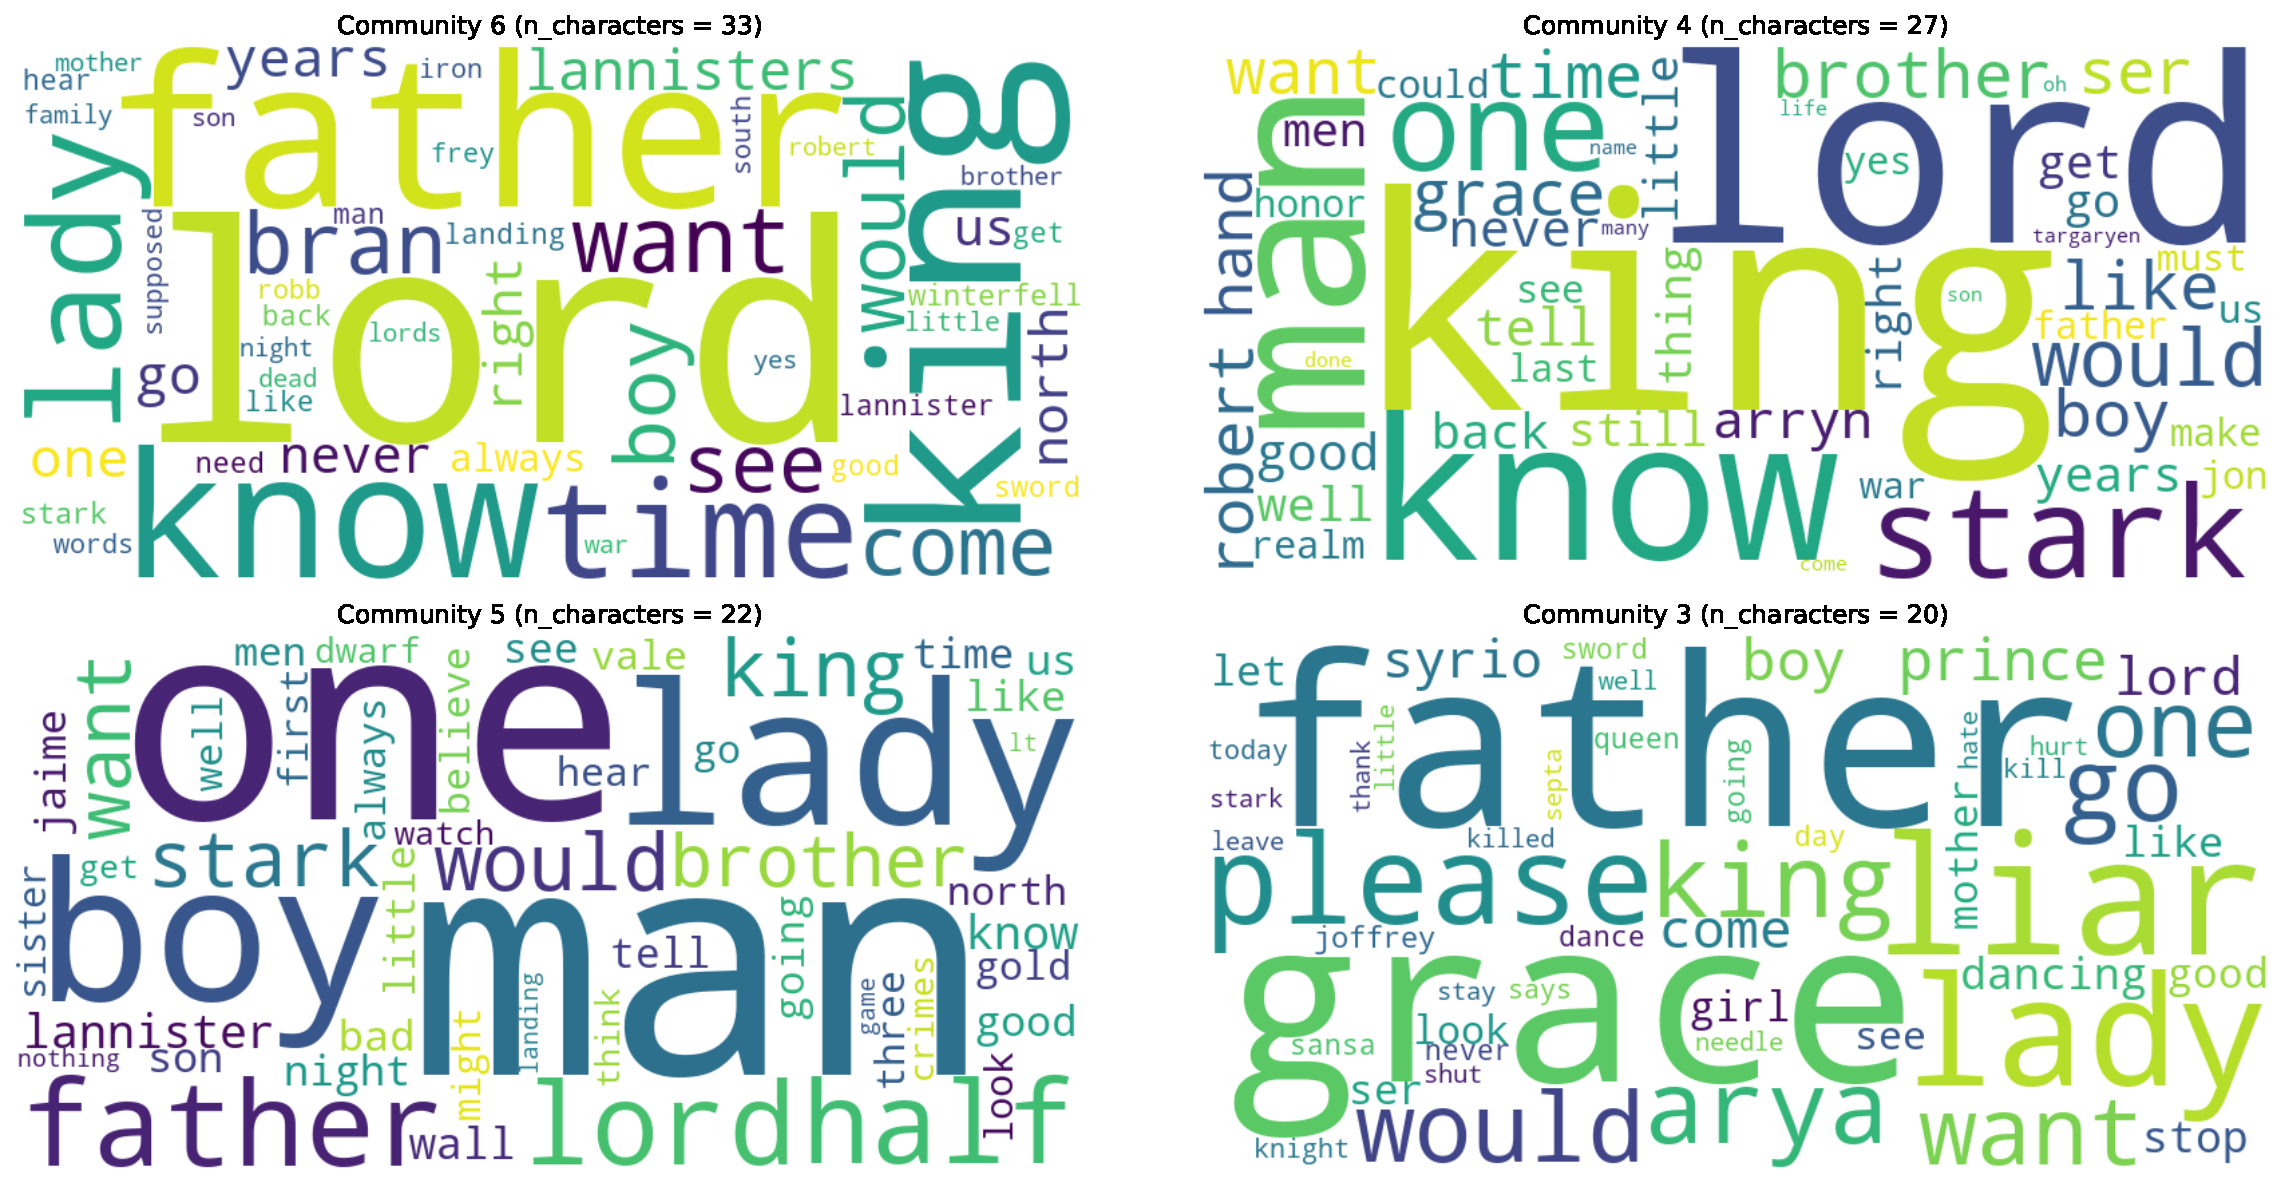
\includegraphics[width=0.9\textwidth]{fig_wordclouds.pdf}
    \caption{Wordclouds of top TF--IDF words for four main communities. Each panel shows the most distinctive words (by TF--IDF) for (A) the Winterfell/Stark community, (B) the King’s Landing community, (C) the Night’s Watch community, and (D) the Dothraki/Daenerys community. The vocabulary reflects family, political, military, and Dothraki-cultural themes, respectively.}
    \label{fig:wordclouds}
\end{figure*}

\subsection*{Sentiment across communities}

To quantify emotional tone, I use the LabMT happiness lexicon by Dodds \emph{et al.}~\cite{dodds2011}, which assigns a happiness score (1--9) to frequent English words. Following standard practice, I exclude neutral words (scores between 4 and 6) and compute, for each community document, a mean happiness score and a shifted version where 0 corresponds to neutral speech.

Community-level sentiment differences are small but systematic. Most large communities have positive shifted scores in the range $0.21$--$0.48$, reflecting a mix of everyday dialogue and dark themes. King’s Landing and the Stark war-related communities tend to use more emotionally charged language around honor, betrayal, and violence, slightly lowering their average happiness compared to the Night’s Watch and Dothraki clusters. Very small communities (e.g., minor children or side characters) show unstable scores due to low token counts.

Figure~\ref{fig:sentiment} summarizes the LabMT sentiment per community. The key observation is not that any community is “happy” or “sad” in an absolute sense, but that the communities discovered from structure alone differ in the emotional coloration of their language in ways that align with plot function.

\begin{figure}[t!]
    \centering
    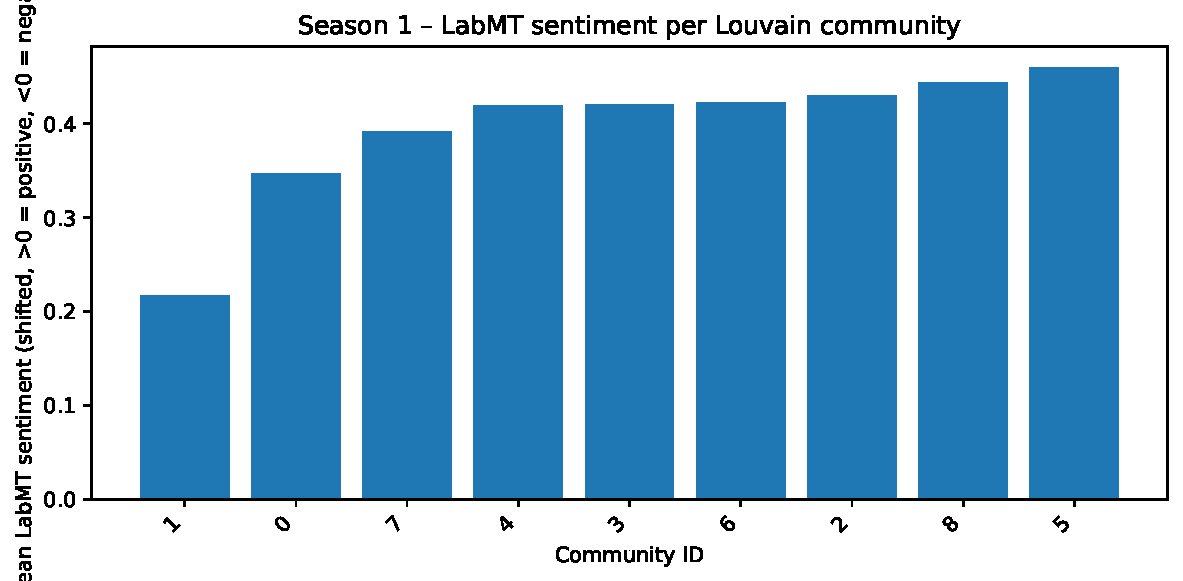
\includegraphics[width=0.9\columnwidth]{fig_sentiment.pdf}
    \caption{LabMT sentiment per Louvain community. Bars show the mean shifted LabMT score (0 = neutral, higher = more positive language) for each community.}
    \label{fig:sentiment}
\end{figure}

%%%%%%%%%%%%%%%%%%%%%%%%%%%%%%%%%%%%%%%%%%%%%%%%%%%%
% Discussion
%%%%%%%%%%%%%%%%%%%%%%%%%%%%%%%%%%%%%%%%%%%%%%%%%%%%

\section*{Discussion}

This project demonstrates how a single Season~1 script dataset can be turned into a complete network--and--text pipeline aligned with a social graphs course. The main findings are:

\begin{itemize}
    \item The Season~1 character interaction network is a single connected component with a skewed degree distribution and clear community structure.
    \item Centrality measures highlight the same characters that narrative intuition would suggest (Eddard, Catelyn, Tyrion, Cersei, Jon, Robb), providing a quantitative confirmation of their importance.
    \item Louvain communities correspond to recognizable factions (Winterfell, King’s Landing, Night’s Watch, Dothraki), and the dominant vocabulary of each group matches its narrative setting and concerns.
    \item Community-level sentiment, measured via LabMT, shows subtle but interpretable differences: communities engaged in political intrigue or war tilt slightly more negative than those focused on training or cultural introduction.
\end{itemize}

From a methodological perspective, the pipeline showcases how relatively simple tools---NetworkX for graph analytics, NLTK and scikit-learn for classical NLP, and the LabMT lexicon for sentiment---can be combined into a coherent research story with a clear research question and interpretable results. Compared with more elaborate prior work on GoT networks~\cite{beveridge2016,liu2017}, this project emphasizes transparency and reproducibility in a teaching setting rather than methodological novelty.

There are several limitations. The interaction network assumes that two characters are connected if they exchange dialogue in the same scene and treats all interactions as undirected and equally weighted (or weighted only by frequency). This ignores directionality, intensity, and non-verbal interactions. The sentiment analysis is lexicon-based and context-free, which is known to miss sarcasm and complex emotions, especially in dark fantasy settings. Finally, the analysis focuses only on Season~1; including later seasons would reveal how communities evolve as the story expands~\cite{breja2021}.

Nevertheless, the core message is robust: \emph{network structure, lexical themes, and sentiment are aligned and jointly reflect the narrative architecture of Season~1}. This makes the GoT universe an engaging playground for teaching concepts from complex networks and text mining, and it suggests similar pipelines for analyzing other narrative worlds or real-world social systems.

%%%%%%%%%%%%%%%%%%%%%%%%%%%%%%%%%%%%%%%%%%%%%%%%%%%%
% Methods
%%%%%%%%%%%%%%%%%%%%%%%%%%%%%%%%%%%%%%%%%%%%%%%%%%%%

\matmethods{

\subsection*{Dataset and preprocessing}

I use a public \emph{Game of Thrones} script dataset from Kaggle~\cite{gotkaggle}, which contains episode metadata (season, episode title) and character-level dialogue. I restrict the data to Season~1 episodes. Character names are normalized by lowercasing and simple string cleaning (e.g., trimming whitespace, merging obvious duplicates). Stage directions and non-dialogue lines are excluded.

\subsection*{Network construction}

Nodes represent unique character names (speakers). For each scene, I consider the ordered list of speakers and add an undirected edge between each pair of distinct speakers who exchange at least one line in that scene. Multiple exchanges increment the edge weight. Self-loops are removed. The resulting Season~1 graph has 146 nodes and 482 edges. All network analysis is implemented in Python using NetworkX~\cite{hagberg2008}.

\subsection*{Global statistics and centralities}

I compute basic statistics (number of nodes, number of edges, density, connected components, size of the largest component, degree distribution) using standard NetworkX functions. Degree, betweenness (with default shortest-path weighting), and eigenvector centrality are used to identify central characters. Rankings are compared across measures and visualized as bar plots.

\subsection*{Community detection}

Communities are detected using the Louvain algorithm~\cite{blondel2008}, as implemented in the \texttt{python-louvain} package. I treat the graph as unweighted for the community detection step, following common practice in the literature. Modularity and community sizes are reported, and nodes are colored by community in visualizations.

\subsection*{Text aggregation and TF--IDF}

For each character, I collect all dialogue lines from Season~1. To construct community-level documents, I aggregate the lines of all characters assigned to a given community. Text is lowercased, tokenized with NLTK~\cite{bird2009}, and stripped of punctuation. I use scikit-learn’s \texttt{TfidfVectorizer} to compute TF--IDF across communities, with English stopwords removed and a minimum document frequency of 2. For each community, I extract the top TF--IDF words and visualize them as wordclouds using the \texttt{wordcloud} library.

\subsection*{Sentiment analysis with LabMT}

I load the English LabMT lexicon of word-level happiness scores~\cite{dodds2011}. Following the original methodology, I drop words with happiness scores between 4 and 6 (neutral band) and compute, for each community document, the mean happiness of the remaining tokens. I then subtract 5 (approximately neutral) to obtain shifted scores used in the figures. Coverage (fraction of tokens with LabMT scores) is reported to qualify the stability of estimates. Communities with very few tokens are interpreted cautiously.

\subsection*{Software and reproducibility}

All analyses are implemented in Python~3 using NetworkX~\cite{hagberg2008}, NLTK~\cite{bird2009}, scikit-learn, and standard plotting libraries. The pipeline is organized in a Jupyter notebook following the week-by-week structure of the DTU 02805 course (network basics, centralities, communities, TF--IDF, and sentiment).}

\showmatmethods{}

%%%%%%%%%%%%%%%%%%%%%%%%%%%%%%%%%%%%%%%%%%%%%%%%%%%%
% Data availability and acknowledgments
%%%%%%%%%%%%%%%%%%%%%%%%%%%%%%%%%%%%%%%%%%%%%%%%%%%%

\dataavail{The script dataset used in this study is publicly available on Kaggle (\emph{Game Of Thrones TV Series script data}~\cite{gotkaggle}). Processed data, analysis scripts, and figure-generating code used in this paper are available in the GitHub repository \url{https://github.com/basharbd/02805-got-social-graphs}.}

\acknow{I thank the instructors and teaching assistants of DTU course 02805 \emph{Social Graphs and Interactions} for providing the conceptual framework and weekly notebooks that inspired the design of this project, as well as my fellow students for helpful discussions.}

\showacknow{}

%%%%%%%%%%%%%%%%%%%%%%%%%%%%%%%%%%%%%%%%%%%%%%%%%%%%
% References
%%%%%%%%%%%%%%%%%%%%%%%%%%%%%%%%%%%%%%%%%%%%%%%%%%%%

\begin{thebibliography}{99}

\bibitem{newman2010}
M.~E.~J. Newman,
\newblock {\em Networks: An Introduction}.
\newblock (Oxford University Press, 2010).

\bibitem{barabasi2016}
A.-L. Barab{\'a}si,
\newblock {\em Network Science}.
\newblock (Cambridge University Press, 2016).

\bibitem{bird2009}
S.~Bird, E.~Klein, E.~Loper,
\newblock {\em Natural Language Processing with Python}.
\newblock (O'Reilly Media, 2009).

\bibitem{dodds2011}
P.~S. Dodds, et~al.,
\newblock Temporal patterns of happiness and information in a global social network.
\newblock {\em PLoS ONE} \textbf{6}(12), e26752 (2011).

\bibitem{hagberg2008}
A.~A. Hagberg, D.~A. Schult, P.~J. Swart,
\newblock Exploring network structure, dynamics, and function using NetworkX.
\newblock In {\em Proceedings of the 7th Python in Science Conference (SciPy)}, pp. 11--15 (2008).

\bibitem{blondel2008}
V.~D. Blondel, J.-L. Guillaume, R.~Lambiotte, E.~Lefebvre,
\newblock Fast unfolding of communities in large networks.
\newblock {\em Journal of Statistical Mechanics: Theory and Experiment} \textbf{2008}(10), P10008 (2008).

\bibitem{beveridge2016}
A.~Beveridge, J.~Shannon,
\newblock The Network of Thrones.
\newblock {\em Math Horizons} \textbf{23}(4), 18--22 (2016).

\bibitem{liu2017}
J.~Liu, et~al.,
\newblock A network analysis of ``Game of Thrones''.
\newblock {\em International Journal of Modern Physics C} \textbf{28}(05), 1750064 (2017).

\bibitem{breja2021}
S.~Breja, et~al.,
\newblock A social network analysis of \emph{Game of Thrones}.
\newblock In {\em 2021 International Conference on Data Analytics for Business and Industry} (2021).

\bibitem{gotkaggle}
G.~Gopinath,
\newblock Game Of Thrones TV Series script data.
\newblock Kaggle dataset (accessed 2025).

\end{thebibliography}

\subsubsection*{Use of Generative AI}
\addcontentsline{toc}{subsection}{Use of Generative AI}

The generative AI tools I have used: ChatGPT (OpenAI, GPT-5.1 ), Which were used to help brainstorm the project design, structure the notebook( plotting, TF-IDF,  loops), and to rephrase parts of the report text.



I reviewed, adapted, and tested all suggested code before using it, and edited to match my own understanding and the actual results. 

All final design decisions, experiments, and interpretations are my own responsibility.


\end{document}
